% !TEX encoding = Windows Cyrillic
\documentclass[a4paper,11pt]{article}
\usepackage{newlistok}

\УвеличитьШирину{1.5cm}
\УвеличитьВысоту{2.5cm}
%\vspace*{1.0cm}

\newcommand{\har}{\mathop{\mathrm{char}}\nolimits}
\renewcommand{\spacer}{}

\renewcommand{\C}{{\mathbb C}}
\newcommand{\Zp}{{\mathbb Z}_p}
\renewcommand{\Z}{\mathbb Z}
\renewcommand{\Q}{\mathbb Q}
\renewcommand{\R}{\mathbb{R}}
%\newcommand{\QT}{{\Q[\sqrt{\raisebox{0ex}[1.35ex]{$2$}}]}}
\newcommand{\QT}{\Q[\sqrt{2}]}
\newcommand*{\longermapsto}{\mathop{\mapstochar\relbar\mskip-10.5mu\rightarrow}}


\newcommand{\ci}{^{\circ}}
\newcommand{\s}{\sin}
\renewcommand{\r}{\sqrt}
\renewcommand{\f}[2]{\left(\frac{#1}{#2}\right)}
\newcommand{\sk}[1]{\left({#1}\right)}
\newcommand{\fr}{\frac}
\renewcommand{\c}{\cos}
\renewcommand{\t}{\tg}
\newcommand{\ct}{\ctg}
\renewcommand{\a}{\alpha}
\renewcommand{\b}{\beta}
\newcommand{\e}{\epsilon}
\newcommand{\w}{\widetilde}
\newcommand{\g}{\gamma}
\renewcommand{\d}{\dfrac}
\renewcommand{\le}{\leqslant}
\renewcommand{\ge}{\geqslant}
\renewcommand{\phi}{\varphi}
\renewcommand{\l}[2]{\log_{#1}#2}
\newcommand{\sns}{\mskip-.5mu}

%\renewcommand*{\hm}[1]{#1\nobreak\discretionary{}%
%{\hbox{$\mathsurround=0pt #1$}}{}}
%

\begin{document}

\НомерЛистка{GT-1}
\Заголовок{Устойчивые паросочетания.}
\ДатаЛистка{2022.01}

\СоздатьЗаголовок

\раздел{Введение}

{\footnotesize
Теория игр занимается, в основном, двумя разными задачами. Первая --- понять, как действуют экономические агенты (люди, фирмы). Вторая --- понять, как организовать процесс (голосования на выборах, аукционы, разбиения на пары) так, чтобы получить устойчивый и рациональный итог.

В этом листке мы изучим <<задачу о марьяже>> (о том, как переженить мужчин и женщин), это наиболее упрощенная модель формирования двусторонних рынков. Здесь под двусторонним рынком подразумевается некоторая совокупность экономических агентов, которая разбита на два множества, взаимодействующие между собой. Эта конструкция позволяет симулировать (а значит, и исследовать с точки зрения экономики и социологии) самые разнообразные типы взаимодействий: рынок труда (работники и фирмы), образование (школьники/студенты и школы/вузы), распределение нагрузки в интернете (пользователи и сервера), товарооборот в торговле (поставщики и магазины) и так далее. За развитие этой теории Ллойд Шепли и Элвин Рот получили Нобелевскую премию по экономике в 2012 году.

}


\опр
Пусть $M$ --- множество мужчин $A_1$, $A_2$,  $\ldots$, $A_k$; $W$ --- множество женщин $a_1$, $a_2$, $\ldots$ , $a_n$.
\textit{Паросочетанием} называется любое однозначное соответствие из $M$ в $W$, то есть набор пар (мужчина, женщина), в котором мужчины и женщины различны. Пусть у каждого мужчины есть список женщин, упорядоченный по убыванию их “привлекательности” для него. Аналогично, у
каждой женщины есть упорядоченный по тому же принципу список мужчин. Паросочетание называется \textit{неустойчивым}, если некие мужчина $A$ и женщина $a$, не состоящие в браке между собой, оба предпочитают друг друга своим супругам, и \textit{устойчивым}, иначе.
\копр

{\bf Задача о марьяже} заключается в следующем: существует ли устойчивое паросочетание? Более тонкий вопрос: если устойчивых паросочетаний несколько, какое из них надо выбрать?

\задача\label{examp} Опишите устойчивые паросочетания при заданных предпочтениях (в строке написан порядок по убыванию):

\пункт 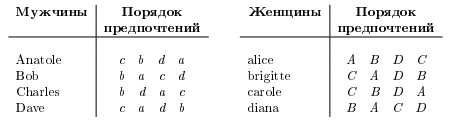
\includegraphics[scale=0.5]{pict1.png};
\пункт 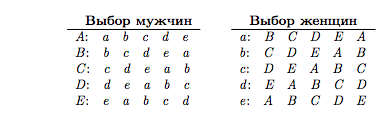
\includegraphics[scale=0.5]{pict2.png}.

\кзадача

\задача[Пример, когда устойчивых паросочетаний много] Приведите пример наборов предпочтений для $N$ мужчин и $N$ женщин, для которых существует $2^{\frac{N}{2}}$ устойчивых паросочетаний. Для простоты можно считать, что $N=2^k$.
\кзадача

\vspace*{-4mm}

\раздел{Алгоритм Гейла-Шепли}

Рассмотрим следующий алгоритм Гейла-Шепли. Вот его $i$-ый шаг:
\\(1) каждый мужчина делает предложение самой привлекательной женщине из тех, кто ещё ему не отказал;
\\(2) каждая женщина отказывает всем мужчинам, сделавшим ей предложение, кроме самого привлекательного для неё.

\задача Примените алгоритм к задаче \ref{examp}. Правда ли, что алгоритм закончит работу и получится устойчивое паросочетание?
\кзадача

\задача
Верно ли, что

\сНовойСтроки

\пункт если женщина $a$ отвергла мужчину $A$, то пара $Aa$ не встретится ни в одном устойчивом паросочетании;

\пункт на каждом шаге алгоритма у любого мужчины список оставшихся предложений не пуст?

\пункт Докажите, что в ходе алгоритма получается устойчивое паросочетание.

\кзадача

\задача Предположим, что мы провели алгоритм Гейла-Шепли и получили устойчивое паросочетание.

\пункт Покажите, что те, кто не попал в это паросочетание (при неравном количестве мужчин и женщин) не попадёт ни в одного другое устойчивое паросочетание.

\пункт Покажите, что данное паросочетание самое лучше (из всех устойчивых паросочетаний) с точки зрения мужчин и самое худшее с точки зрения женщин.
\кзадача

\задача Проведём алгоритм Гейла-Шепли сначала, когда мужчины делают предложения, а женщины отказывают;  а потом --- когда женщины делают предложения, а мужчины отказывают. Пусть получилось одно и тоже паросочетание. Верно ли, что при данных упорядочиваниях устойчивое паросочетание единственно?
\кзадача

%\newpage

\задача Покажите, что алгоритм Гейла-Шепли можно обобщить на случай <<абитуриенты>> --- <<университеты>>. А именно, теперь в одном из множеств (в данном случае, университеты) элементы могут связываться с несколькими абитуриентами. Будем считать, что у каждого университета помимо упорядочивания задача ещё и  \выд{мощность}, то есть количество пар, которые он хочет образовать.
\кзадача

\задача Сколько устойчивых паросочетаний может быть, если мужчин и женщин по три?
\кзадача

\задача Пусть $M = (Aa, Bb, \ldots , Zz)$ и $M_0 = (Aa_0, Bb_0,\ldots , Zz_0)$ --- два произвольных устойчивых паросочетания. Докажите, что набор
$M \vee M_0 = (A \max_A(a,a_0), B \max_B(b,b_0),\ldots, Z \max_Z(z,z_0))$\\ \пункт является паросочетанием; \пункт является устойчивым паросочетанием.
\\
(Здесь $\max_A(a, a_0)$ есть женщина, наиболее предпочтительная для $A$ из двух кандидатур $a$ и $a_0$.)
\\\пункт Докажите аналогичное утверждение про $M \wedge M_0 = (A \min_A(a,a_0), B \min_B(b,b_0),\ldots, Z \min_Z(z,z_0))$.

\кзадача


\ЛичныйКондуит{0mm}{4.5mm}
% \GenXMLW

\end{document} 